% !TeX root = ../praktikum.tex
% !TeX encoding = UTF-8
% !Tex spellcheck = de_DE

Im letzten Versuchsabschnitt wurde der Einfluss einer Gatespannung auf die beiden zu untersuchenden Effekte beleuchtet, mit dem Ziel, aus den dadurch erfassten Daten, den Abstand des 2DEG in der Probe zur Gateelektrode zu bestimmen.

Für die folgenden Messungen wurden in Schritten von \unit[50]{mV} Gatespannungen von $-200$ bis \unit[200]{mV} gewählt. Dabei wurde eine Temperatur von \unit[2]{K} an der Probe eingestellt und analog zu den obigen Versuchsteilen aufgrund der deutlicheren Hall-Plateaus in den Graphen die Wechselstromquelle genutzt. 

Der aus der Hallspannung berechnete Hall-Widerstand ist in Abbildung~\ref{fig:gate_mess} im Messbereich von $0$ bis \unit[7.7]{T} aufgetragen.

\begin{figure}[h]
	\centering
	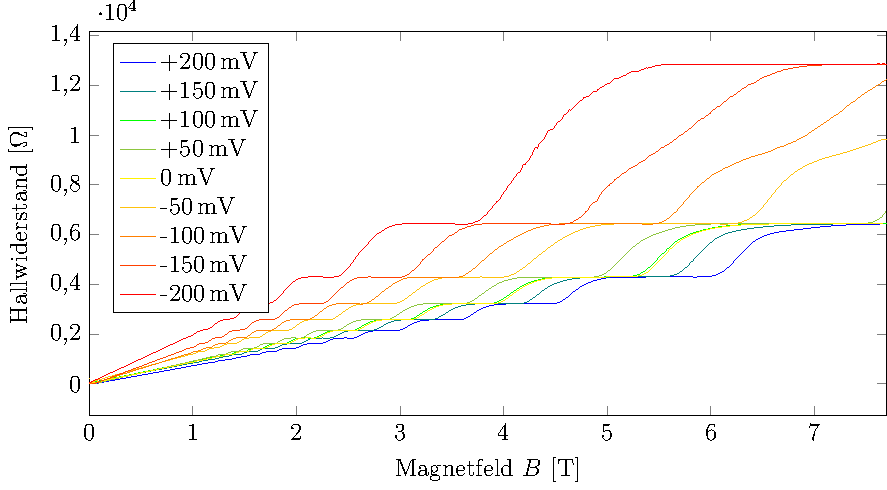
\includegraphics[scale=1]{graphs/gate/full_range.pdf}
	\caption[Auswertung der Gatespannungsvariation]{
		Berechnete Elektronendichte $n_s$ und -beweglichkeit $\mu$ in Abhängigkeit zu der Gatespannung.
	}
	\label{fig:gate_mess}
\end{figure}

